\clearpage
\section{Impact on the proton PDFs}
\label{sec:protonPDFs}

Using the PDF4LHC21~\cite{PDF4LHCWorkingGroup:2022cjn} PDF set, the results are illustrated by comparing the fractional uncertainties of the original PDF set to those obtained after profiling. 
This is shown for the valence quark, gluon and the singlet distributions in Fig.~\ref{FASERv2_profiling} for FASER$\nu$2 pseudodata, while Fig.~\ref{FASERv_profiling} indicates the impact of FASER$\nu$. FASER$\nu$2 is observed to provide tighter constraints on the PDFs, with the effects being the most prominent for the valence and sea quark distributions.

\begin{figure}[H]
\centering
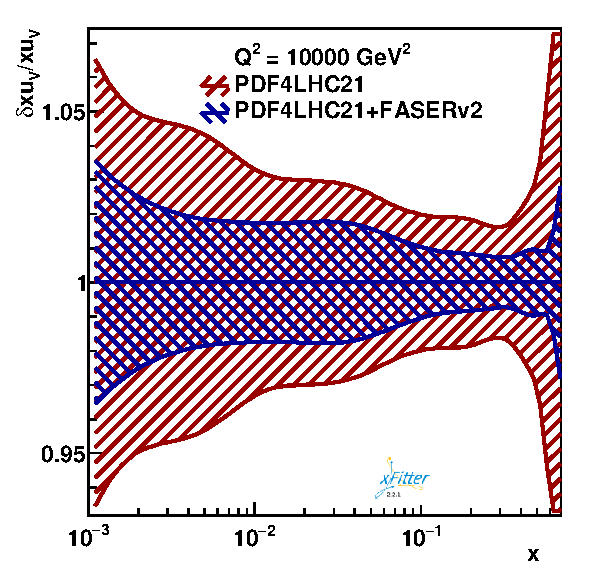
\includegraphics[width=0.4\textwidth]{./figs_xFitter/FASERv2_q2_10000_pdf_uv_ratio.pdf}
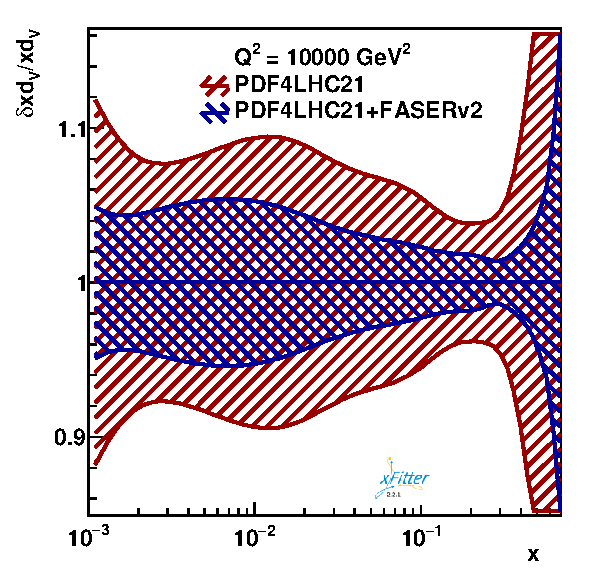
\includegraphics[width=0.4\textwidth]{./figs_xFitter/FASERv2_q2_10000_pdf_dv_ratio.pdf}\\
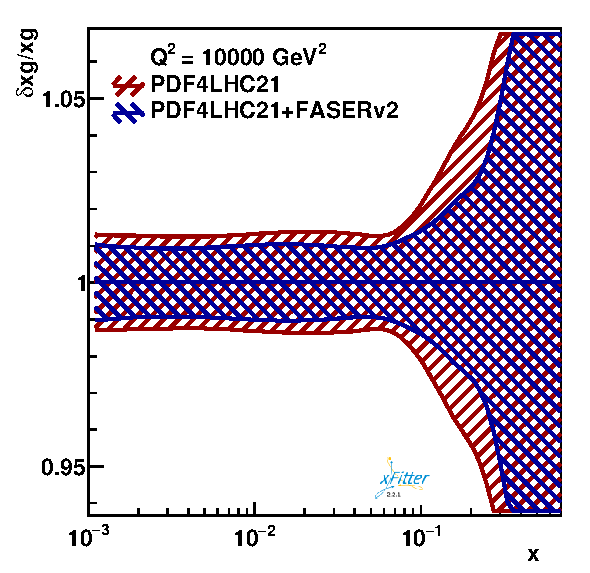
\includegraphics[width=0.4\textwidth]{./figs_xFitter/FASERv2_q2_10000_pdf_g_ratio.pdf}
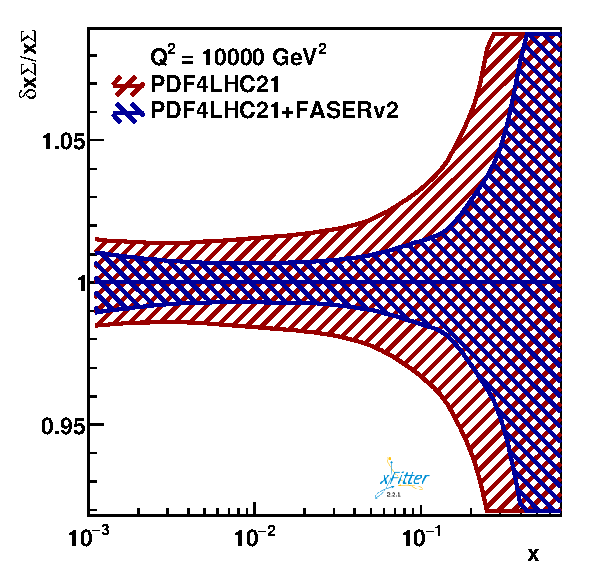
\includegraphics[width=0.4\textwidth]{./figs_xFitter/FASERv2_q2_10000_pdf_Sea_ratio.pdf}
\caption{The fractional uncertainties in the valence quark, gluon and singlet PDFs as a function of the momentum fraction $x$ at the scale $Q^2 = 10000 \, \textrm{GeV}^2$. The profiling is performed using the
PDF4LHC21 set and the pseudodata for FASER$\nu$2. The original uncertainty of PDF4LHC21 is
indicated by the red band, while the blue band demonstrates the profiled result.}
\label{FASERv2_profiling}
\end{figure}

\begin{figure}[H]
\centering
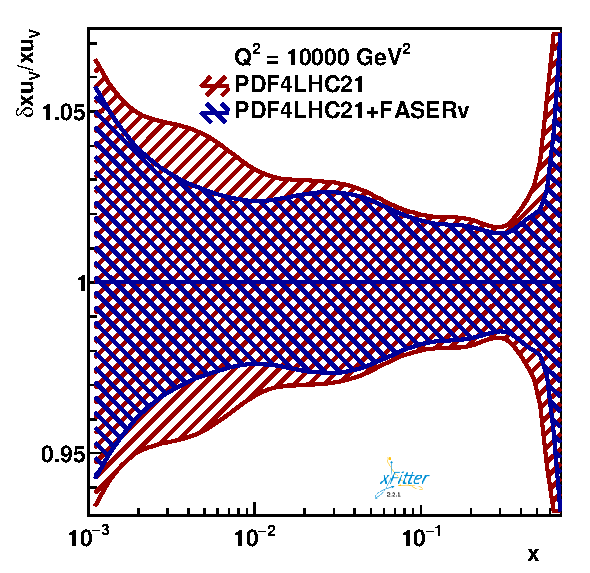
\includegraphics[width=0.4\textwidth]{./figs_xFitter/FASERv_q2_10000_pdf_uv_ratio.pdf}
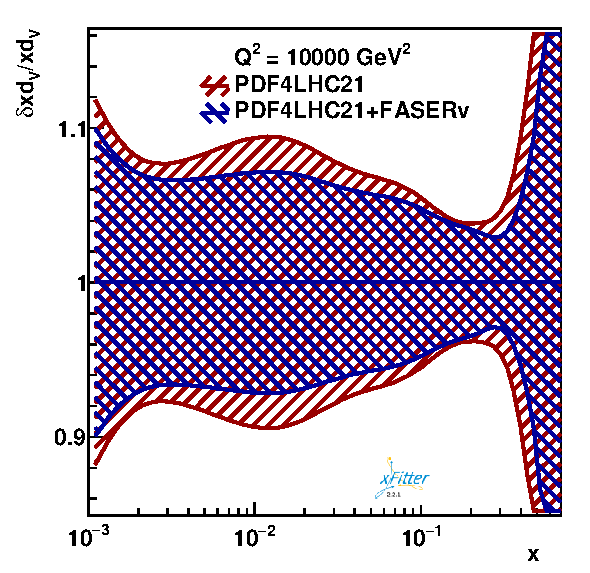
\includegraphics[width=0.4\textwidth]{./figs_xFitter/FASERv_q2_10000_pdf_dv_ratio.pdf}\\
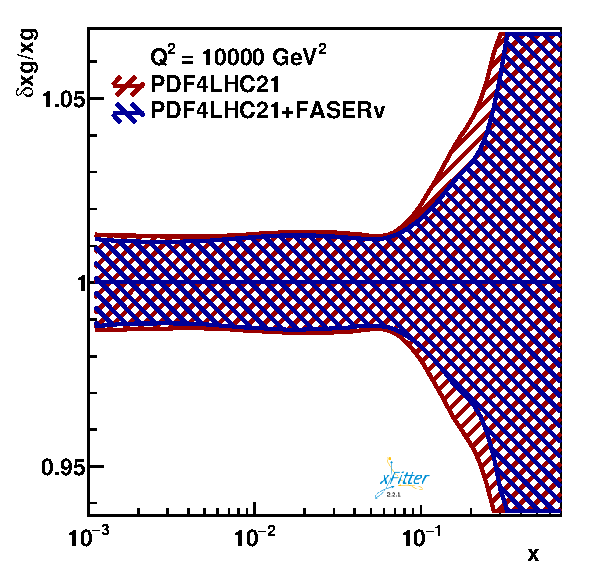
\includegraphics[width=0.4\textwidth]{./figs_xFitter/FASERv_q2_10000_pdf_g_ratio.pdf}
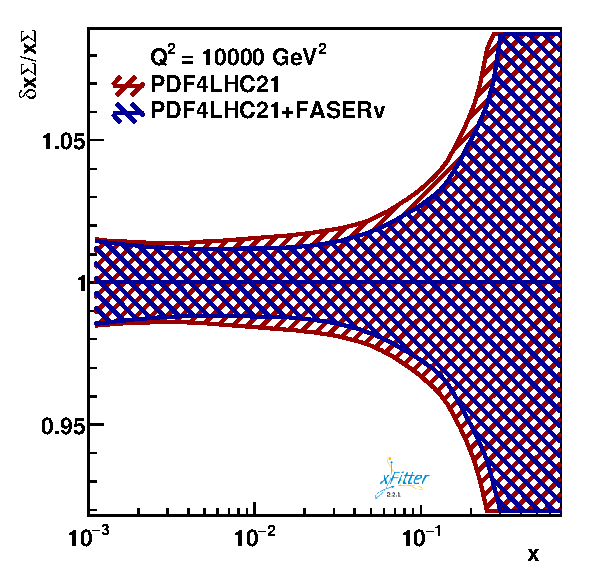
\includegraphics[width=0.4\textwidth]{./figs_xFitter/FASERv_q2_10000_pdf_Sea_ratio.pdf}
\caption{The fractional uncertainties in the valence quark, gluon and singlet PDFs as a function of the momentum fraction $x$ at the scale $Q^2 = 10000 \, \textrm{GeV}^2$. The profiling is performed using the
PDF4LHC21 set and the pseudodata for FASER$\nu$. The original uncertainty of PDF4LHC21 is
indicated by the red band, while the blue band demonstrates the profiled result.}
\label{FASERv_profiling}
\end{figure}


